\documentclass[a4paper,12pt]{article}
\usepackage[utf8]{inputenc}
\usepackage[polish]{babel}
\usepackage{graphicx}
\usepackage{geometry}
\usepackage{hyperref}
\usepackage{float}
\geometry{margin=2.5cm}

\title{Podsumowanie eksperymentów numerycznych\thanks{Automatycznie wygenerowano -- {\today}}}
\author{Autor: Greg}
\date{\today}

\begin{document}
\maketitle
\tableofcontents
\newpage

\section{Wstęp}
Celem niniejszego raportu jest podsumowanie wyników eksperymentów numerycznych przeprowadzonych dla trzech funkcji testowych: kwadratowej, Rosenbrocka oraz Ackleya, w wymiarach $n=10$ oraz $n=30$. Analizowano wpływ parametrów $\sigma$ oraz $a$ na przebieg optymalizacji. Wyniki przedstawiono w postaci wykresów median wartości funkcji celu oraz parametru $\sigma$ w czasie.

\section{Opis eksperymentów}
Dla każdej funkcji i wymiaru przeprowadzono eksperymenty dla kombinacji $\sigma \in \{0.1, 1.0, 10.0\}$ oraz $a \in \{10, 100\}$. Każda konfiguracja była powtarzana 10 razy. Na wykresach zbiorczych przedstawiono mediany przebiegów dla wszystkich kombinacji parametrów.

% --- Quadratic n=10 ---
\section{Funkcja kwadratowa, $n=10$}
\begin{figure}[H]
    \centering
    \begin{minipage}{0.48\textwidth}
        \centering
        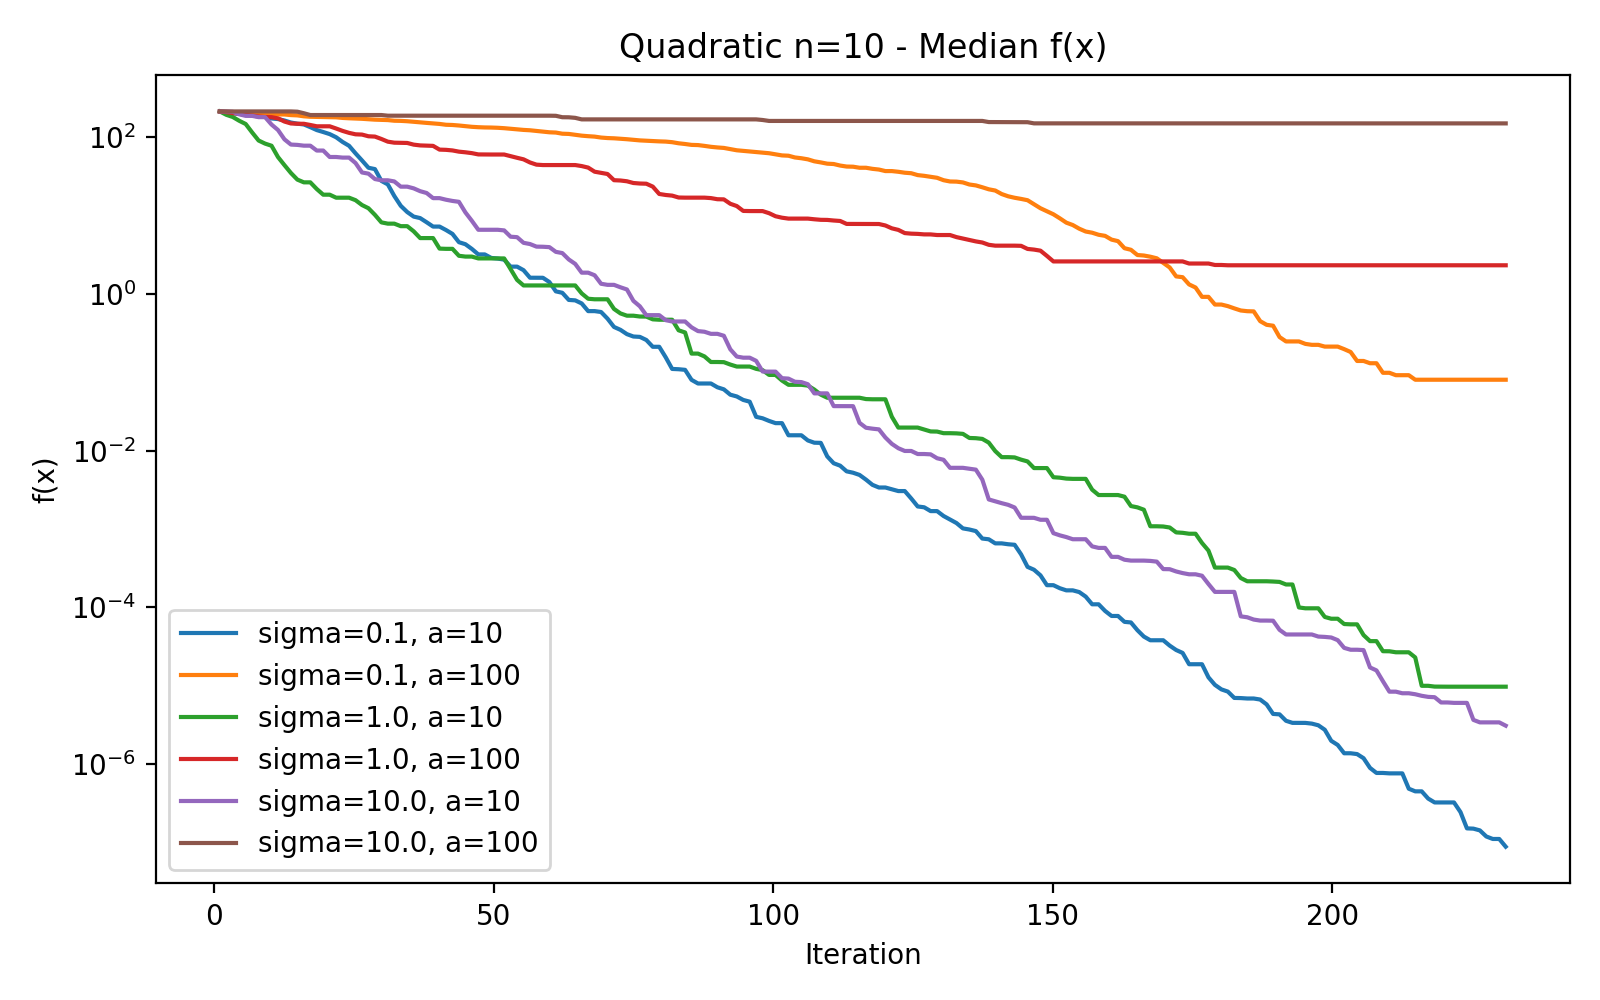
\includegraphics[width=\textwidth]{charts/Quadratic_n10_all_medians.png}\\
        \small Mediany $f(t)$
    \end{minipage}\hfill
    \begin{minipage}{0.48\textwidth}
        \centering
        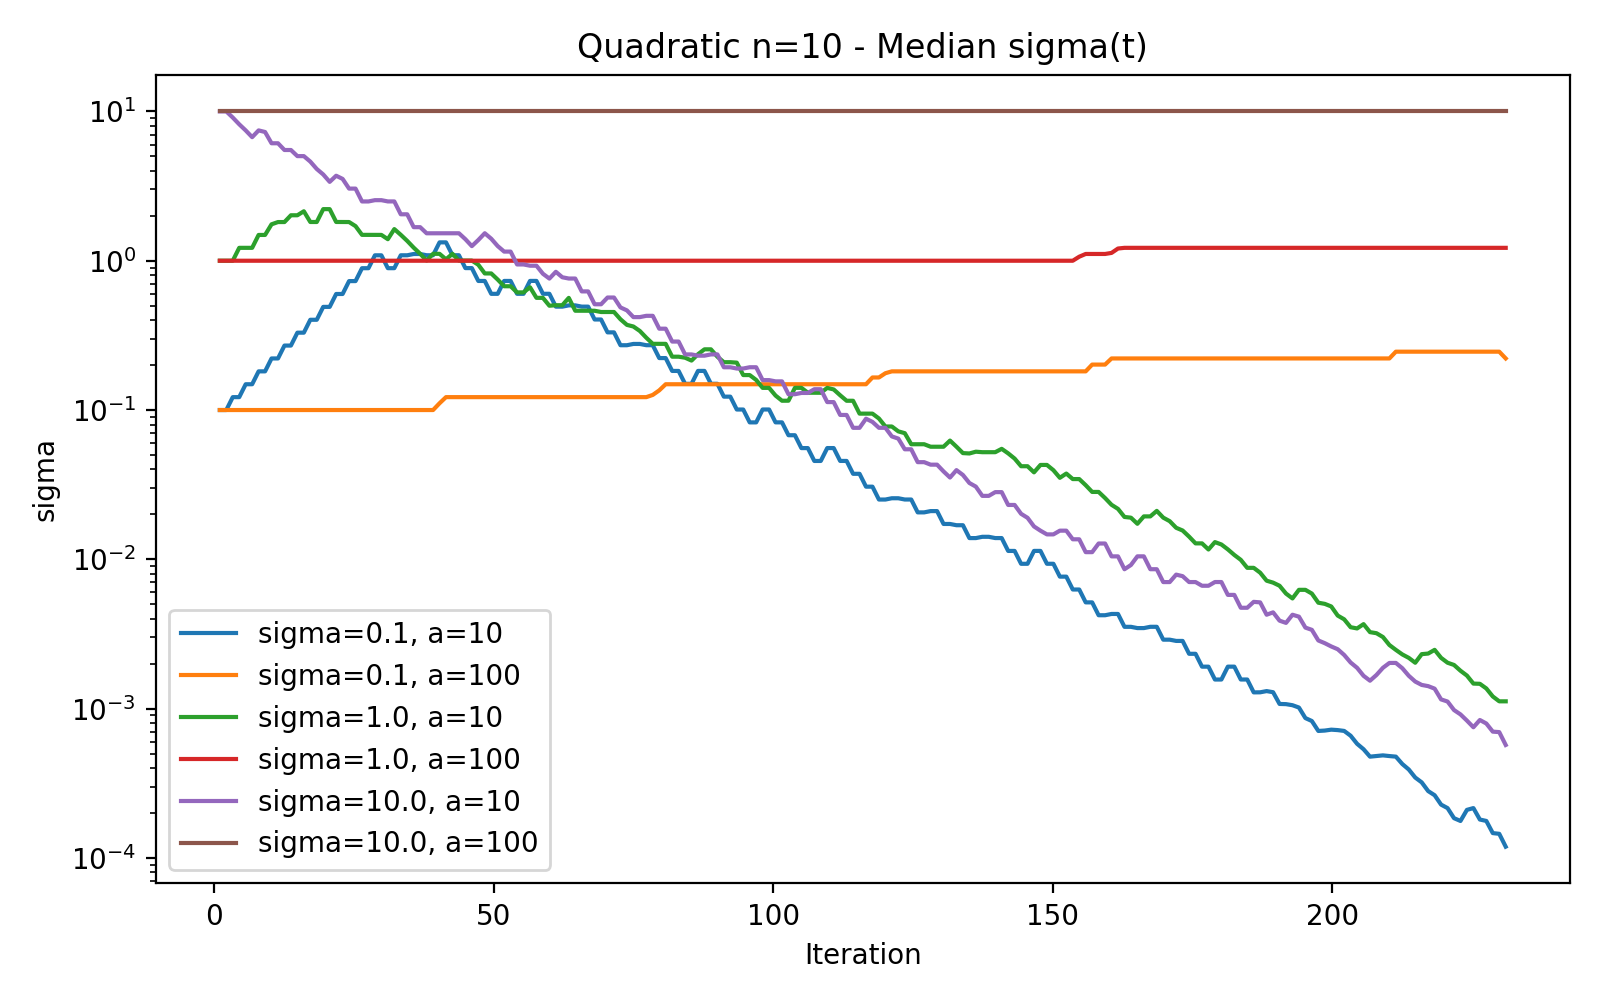
\includegraphics[width=\textwidth]{charts/Quadratic_n10_all_sigmas.png}\\
        \small Mediany $\sigma(t)$
    \end{minipage}
    \caption{Mediany $f(t)$ oraz $\sigma(t)$ dla funkcji kwadratowej ($n=10$) dla różnych $\sigma$ i $a$.}
\end{figure}

% --- Quadratic n=30 ---
\section{Funkcja kwadratowa, $n=30$}
\begin{figure}[H]
    \centering
    \begin{minipage}{0.48\textwidth}
        \centering
        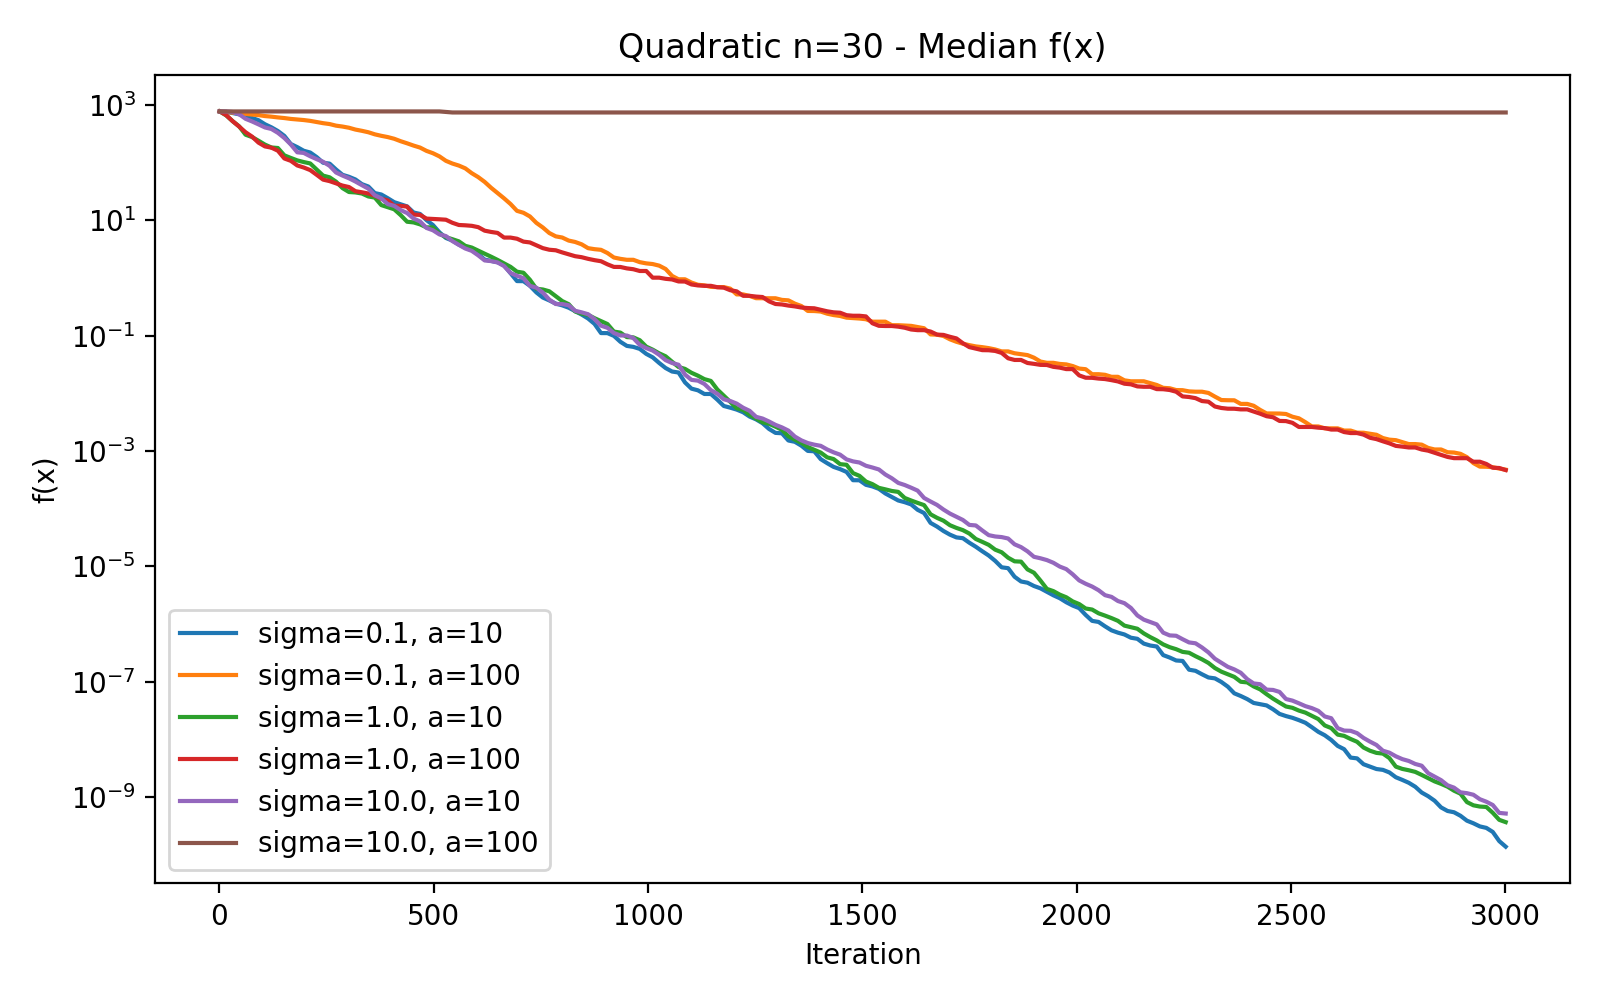
\includegraphics[width=\textwidth]{charts/Quadratic_n30_all_medians.png}\\
        \small Mediany $f(t)$
    \end{minipage}\hfill
    \begin{minipage}{0.48\textwidth}
        \centering
        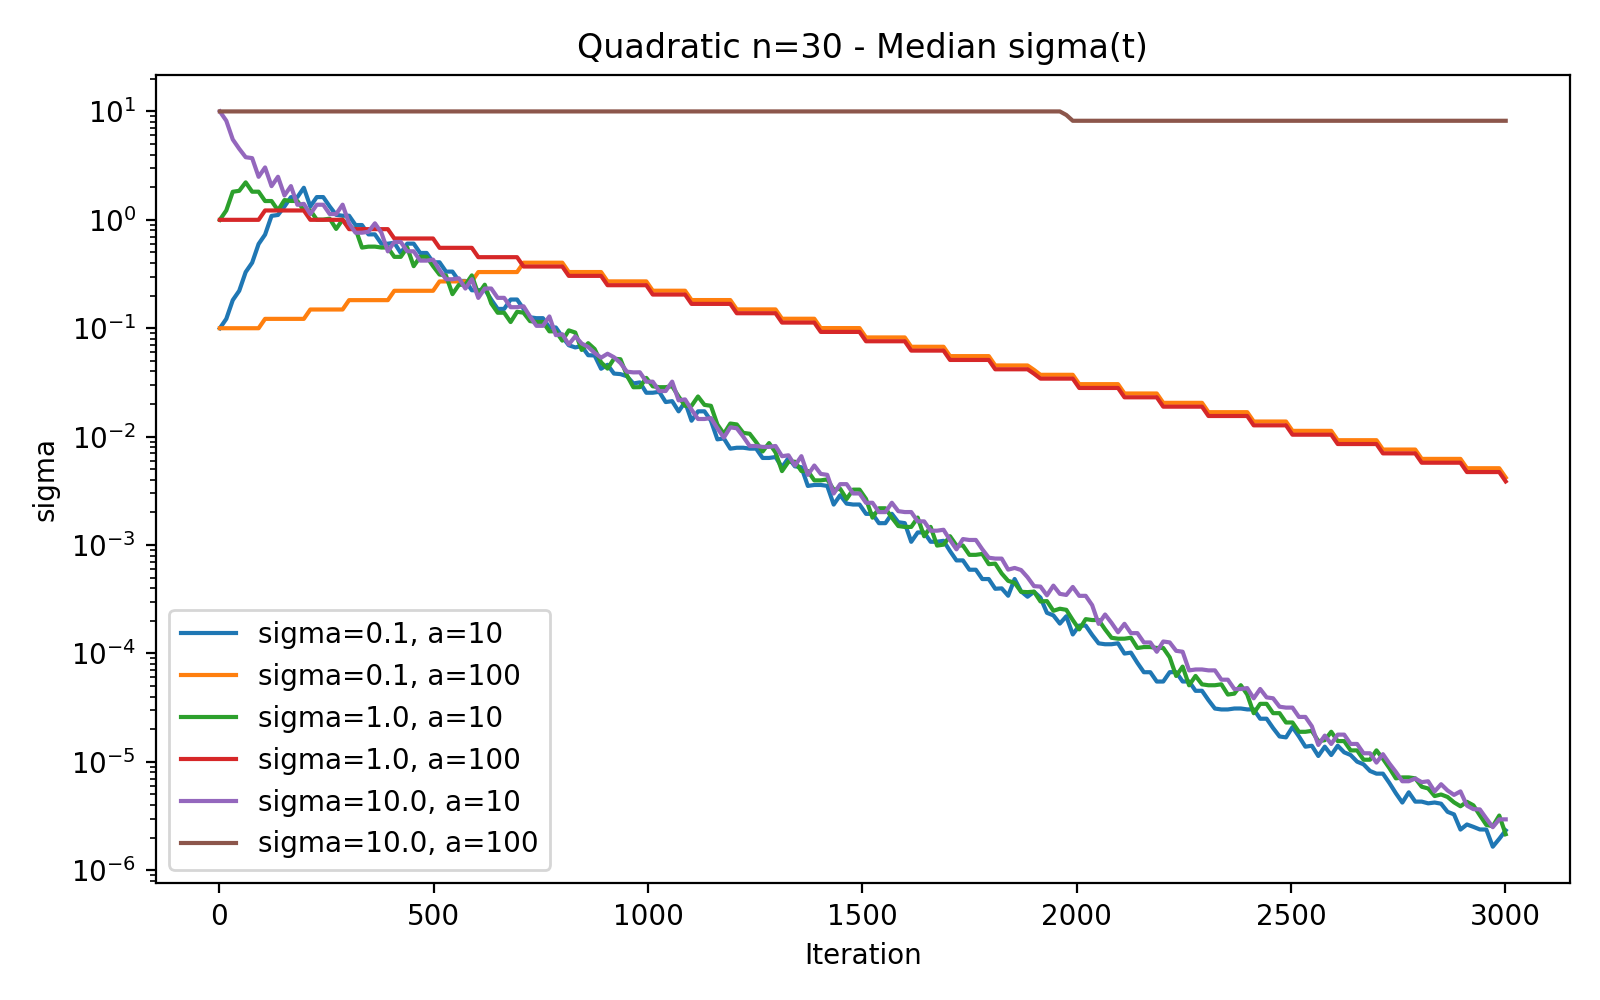
\includegraphics[width=\textwidth]{charts/Quadratic_n30_all_sigmas.png}\\
        \small Mediany $\sigma(t)$
    \end{minipage}
    \caption{Mediany $f(t)$ oraz $\sigma(t)$ dla funkcji kwadratowej ($n=30$) dla różnych $\sigma$ i $a$.}
\end{figure}

% --- Rosenbrock n=10 ---
\section{Funkcja Rosenbrocka, $n=10$}
\begin{figure}[H]
    \centering
    \begin{minipage}{0.48\textwidth}
        \centering
        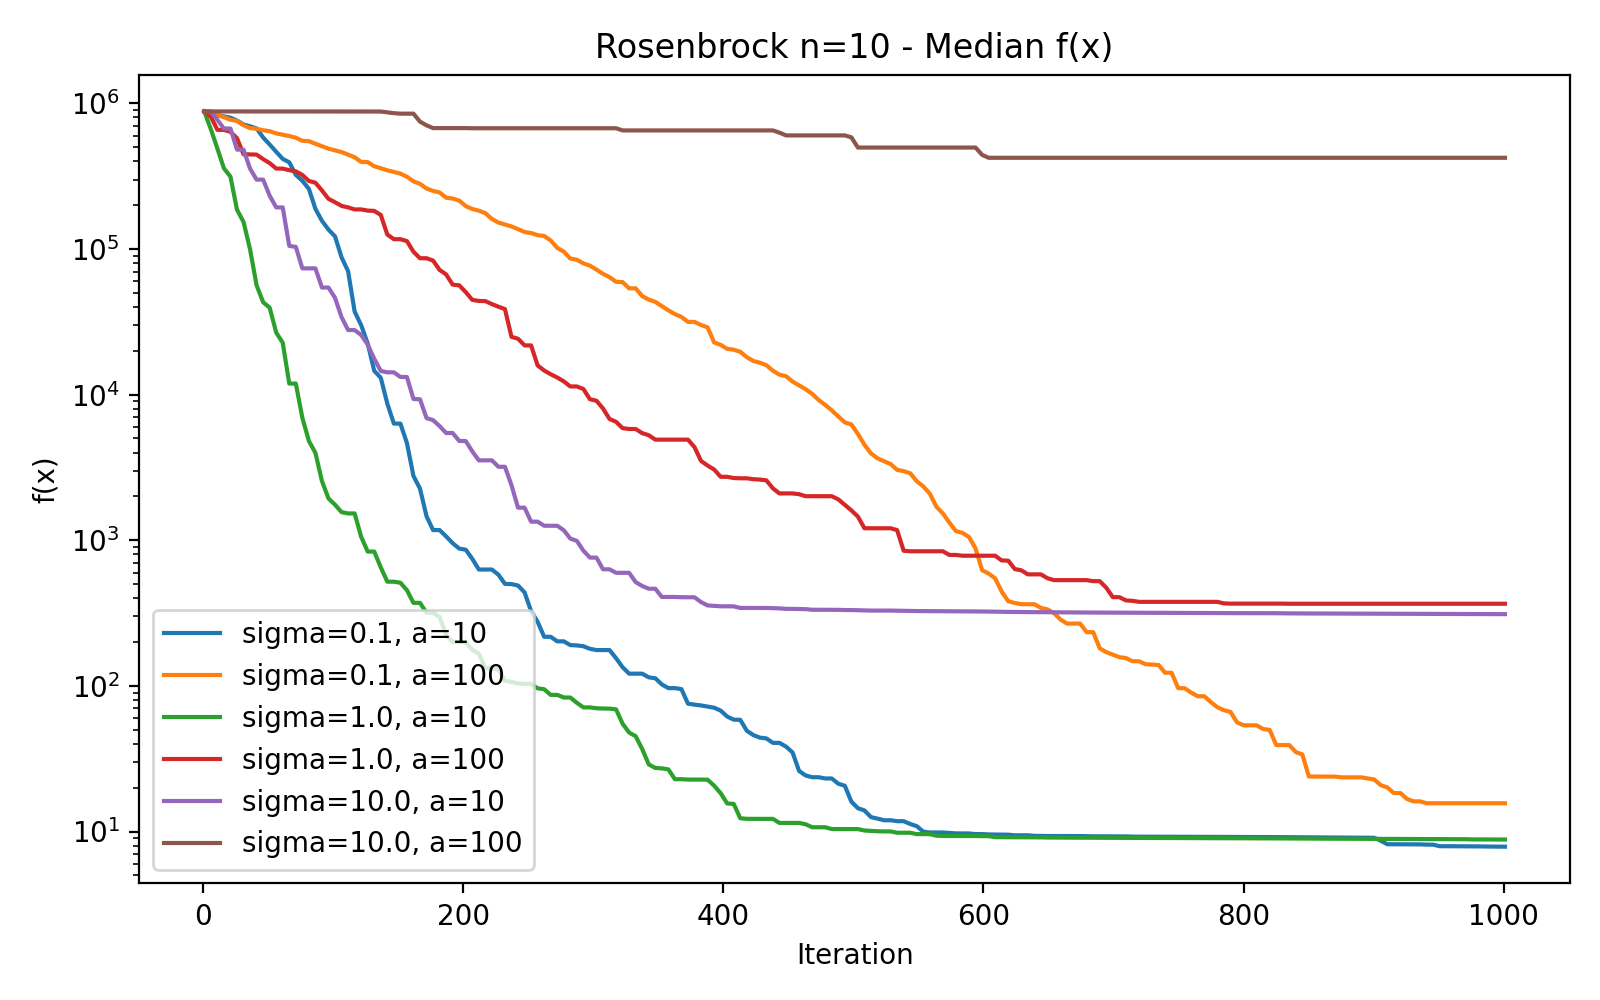
\includegraphics[width=\textwidth]{charts/Rosenbrock_n10_all_medians.png}\\
        \small Mediany $f(t)$
    \end{minipage}\hfill
    \begin{minipage}{0.48\textwidth}
        \centering
        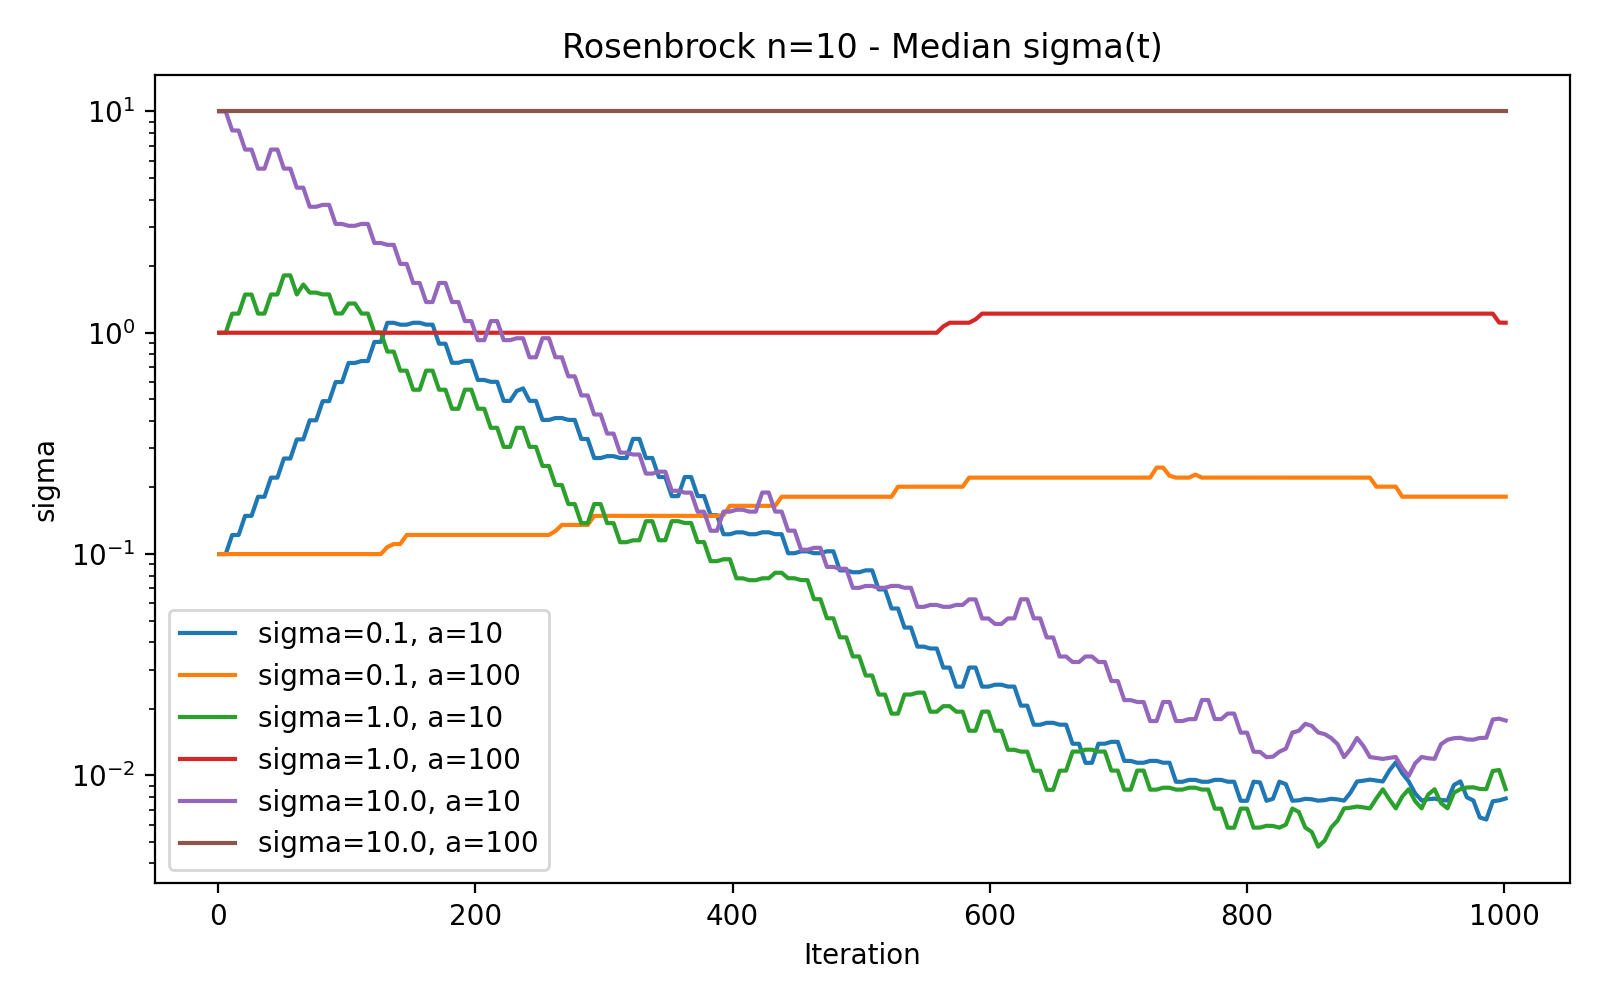
\includegraphics[width=\textwidth]{charts/Rosenbrock_n10_all_sigmas.png}\\
        \small Mediany $\sigma(t)$
    \end{minipage}
    \caption{Mediany $f(t)$ oraz $\sigma(t)$ dla funkcji Rosenbrocka ($n=10$) dla różnych $\sigma$ i $a$.}
\end{figure}

% --- Rosenbrock n=30 ---
\section{Funkcja Rosenbrocka, $n=30$}
\begin{figure}[H]
    \centering
    \begin{minipage}{0.48\textwidth}
        \centering
        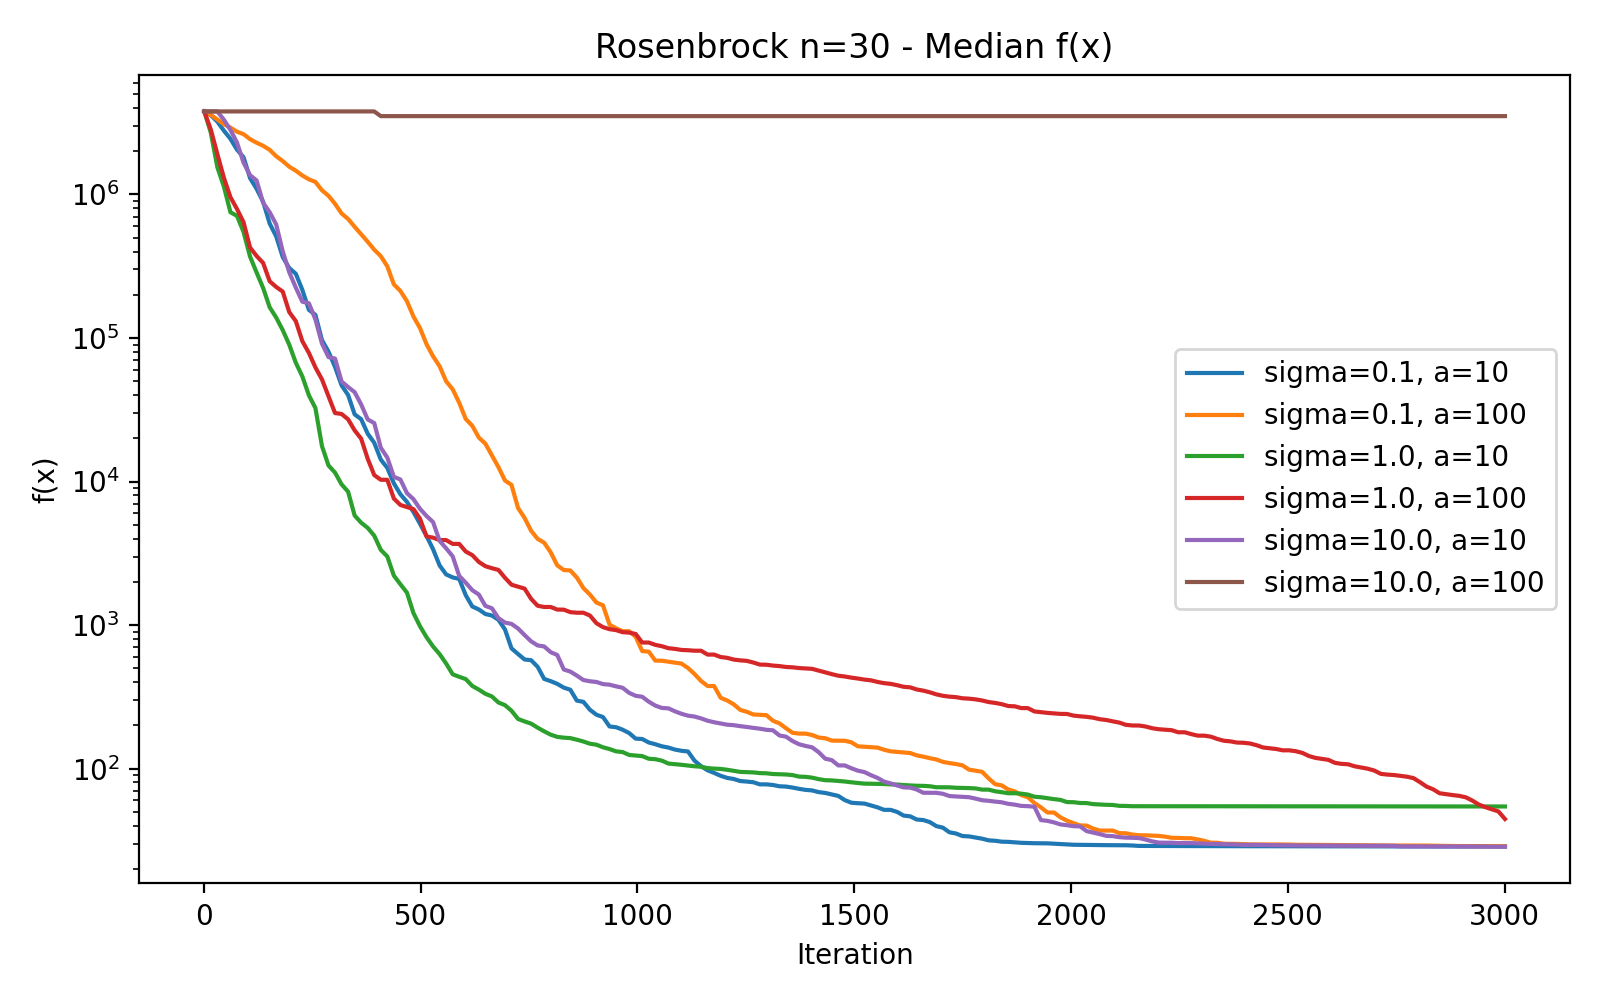
\includegraphics[width=\textwidth]{charts/Rosenbrock_n30_all_medians.png}\\
        \small Mediany $f(t)$
    \end{minipage}\hfill
    \begin{minipage}{0.48\textwidth}
        \centering
        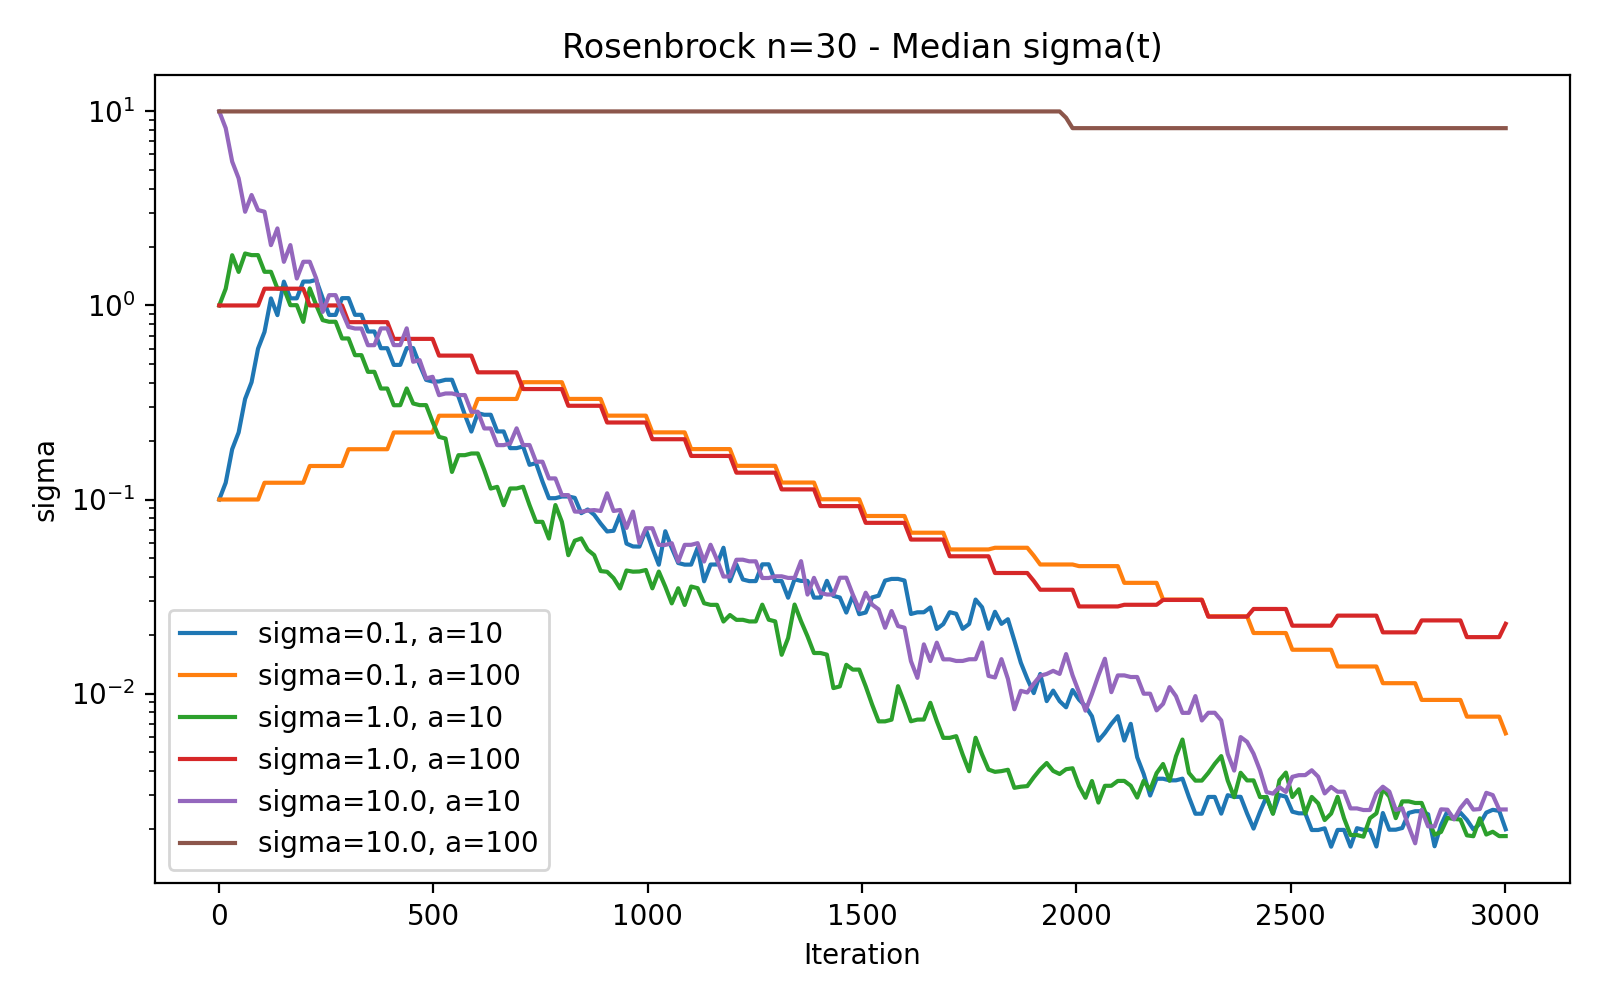
\includegraphics[width=\textwidth]{charts/Rosenbrock_n30_all_sigmas.png}\\
        \small Mediany $\sigma(t)$
    \end{minipage}
    \caption{Mediany $f(t)$ oraz $\sigma(t)$ dla funkcji Rosenbrocka ($n=30$) dla różnych $\sigma$ i $a$.}
\end{figure}

% --- Ackley n=10 ---
\section{Funkcja Ackleya, $n=10$}
\begin{figure}[H]
    \centering
    \begin{minipage}{0.48\textwidth}
        \centering
        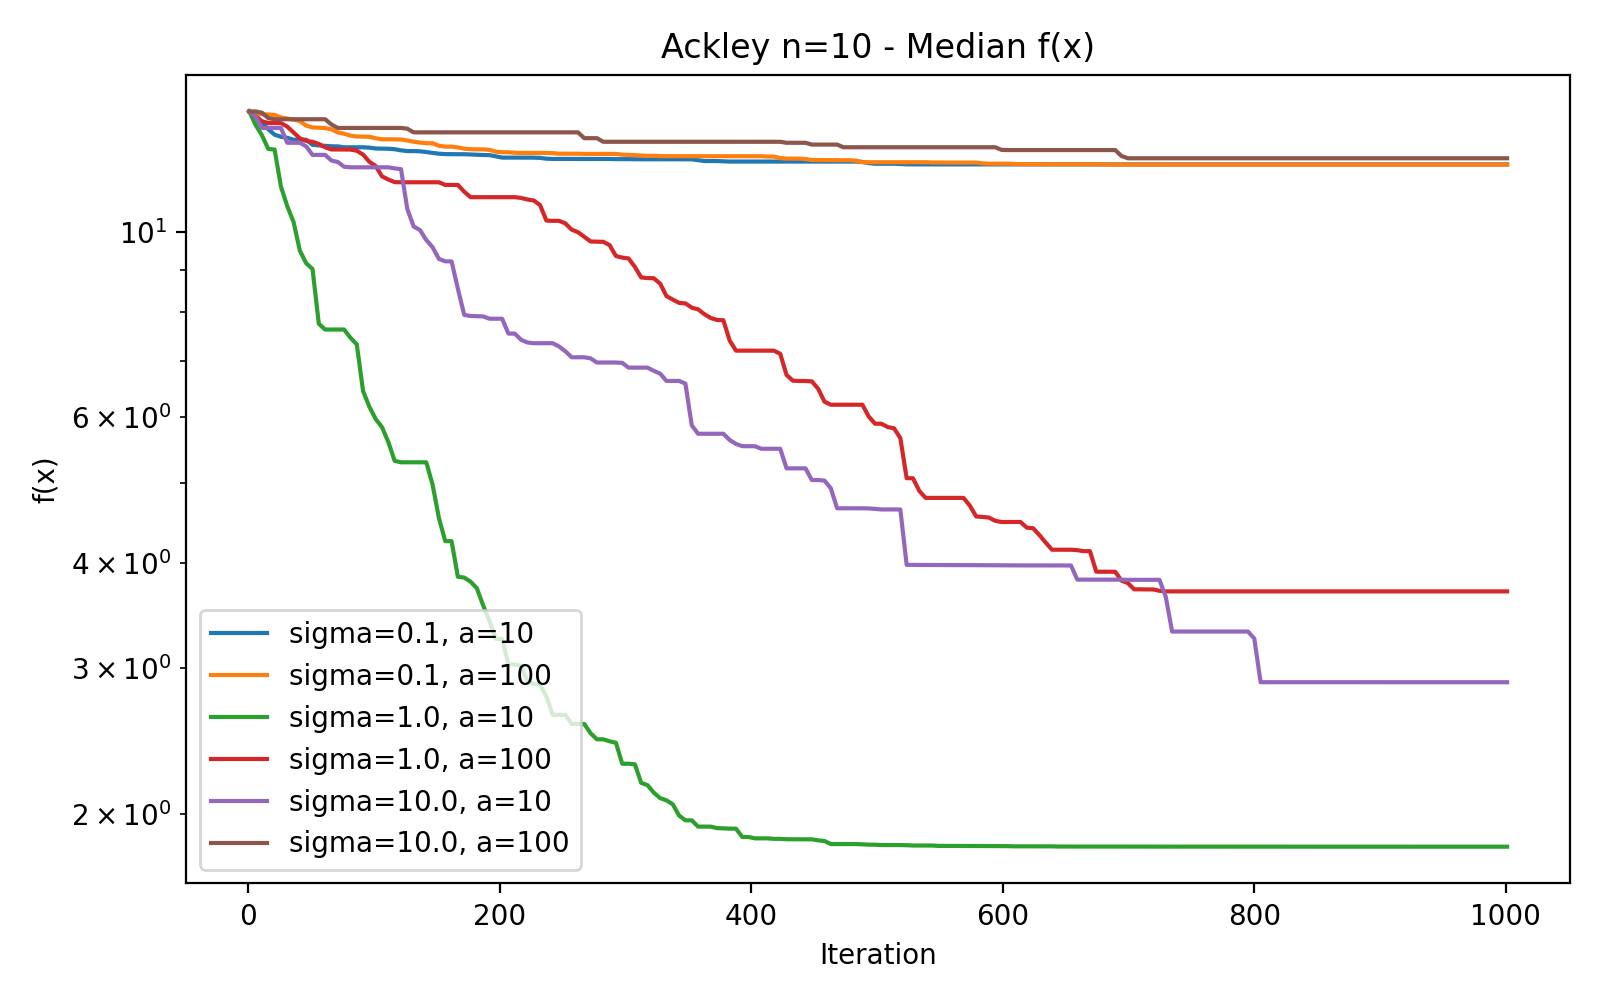
\includegraphics[width=\textwidth]{charts/Ackley_n10_all_medians.png}\\
        \small Mediany $f(t)$
    \end{minipage}\hfill
    \begin{minipage}{0.48\textwidth}
        \centering
        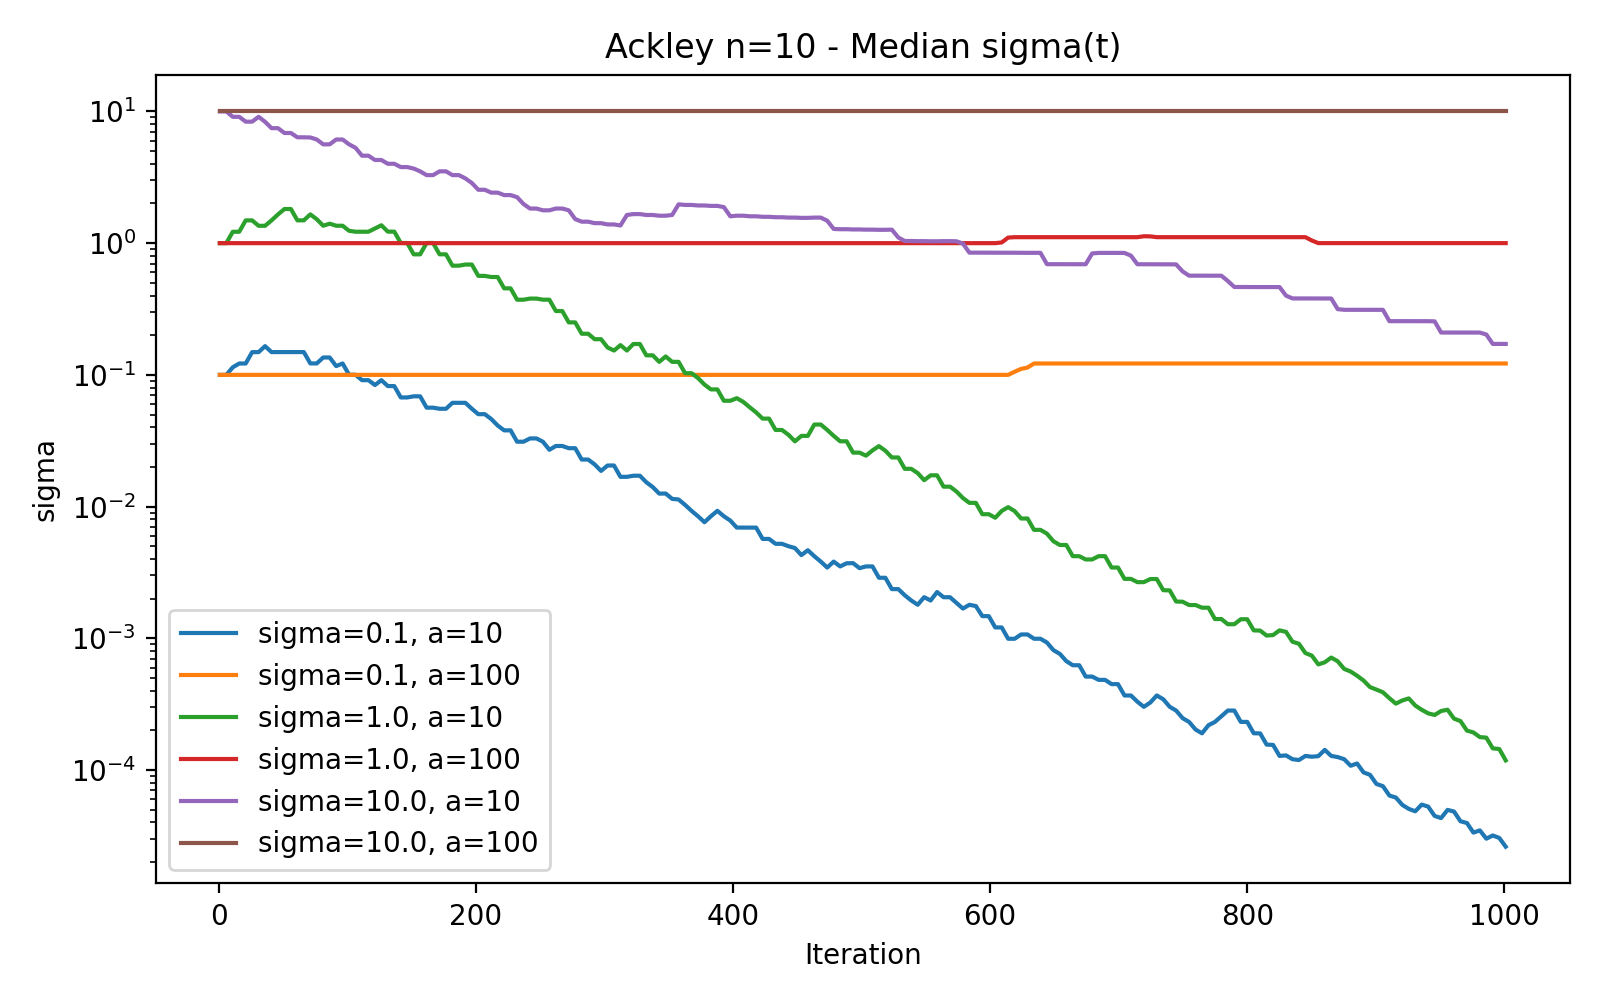
\includegraphics[width=\textwidth]{charts/Ackley_n10_all_sigmas.png}\\
        \small Mediany $\sigma(t)$
    \end{minipage}
    \caption{Mediany $f(t)$ oraz $\sigma(t)$ dla funkcji Ackleya ($n=10$) dla różnych $\sigma$ i $a$.}
\end{figure}

% --- Ackley n=30 ---
\section{Funkcja Ackleya, $n=30$}
\begin{figure}[H]
    \centering
    \begin{minipage}{0.48\textwidth}
        \centering
        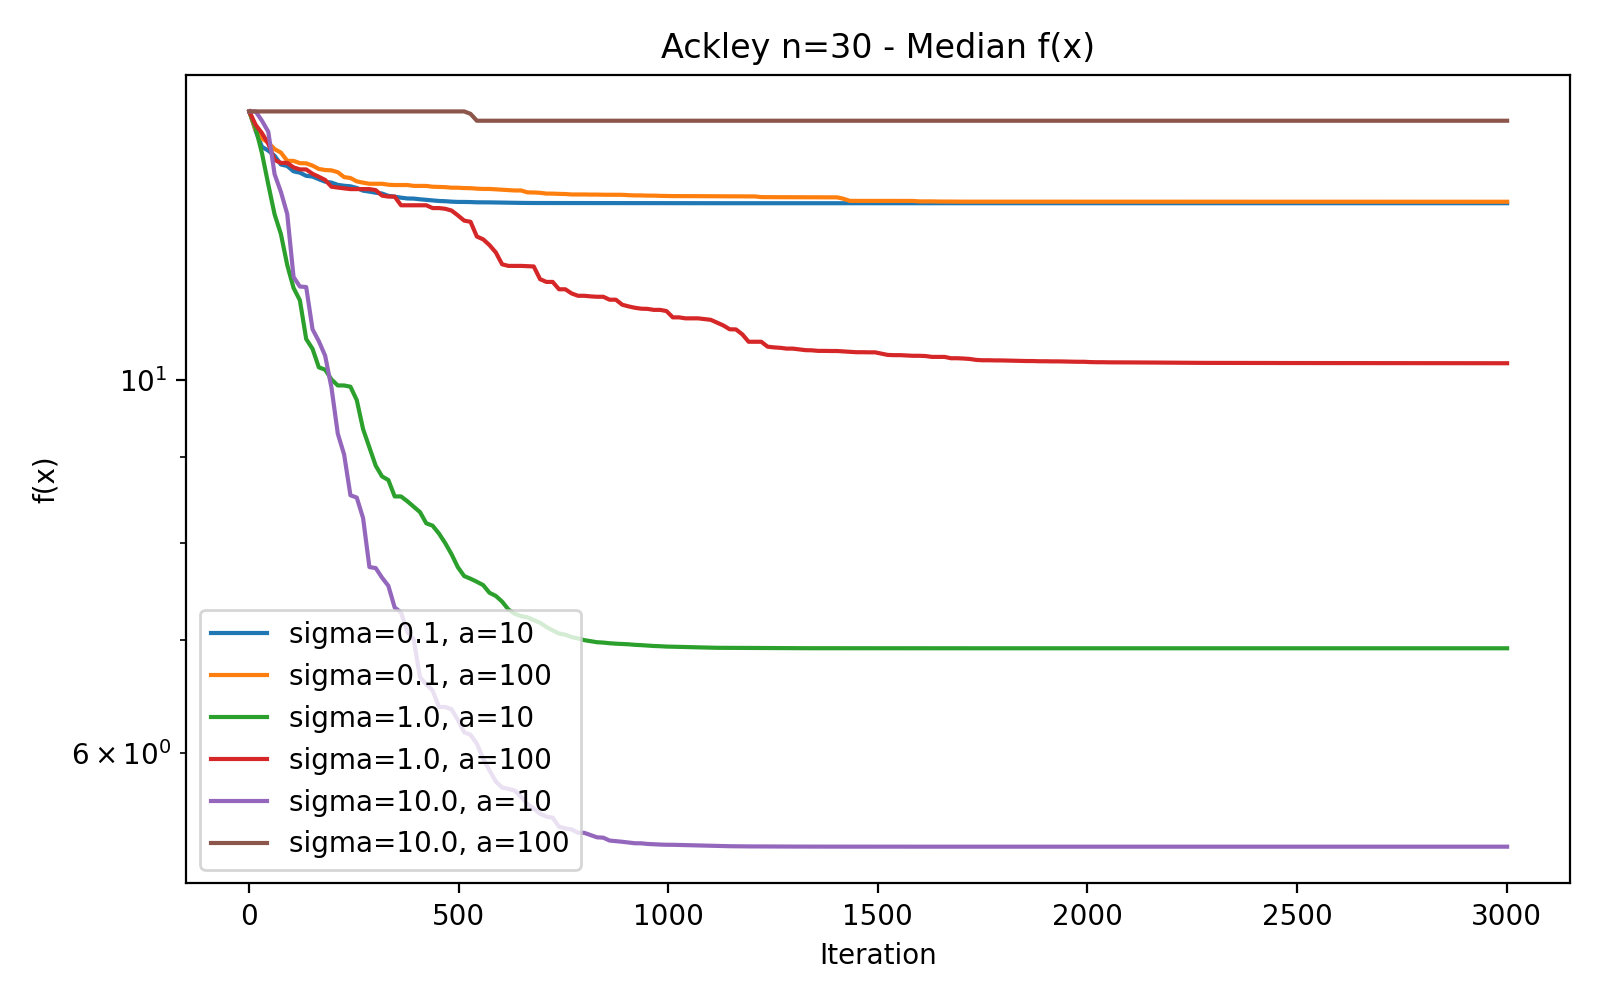
\includegraphics[width=\textwidth]{charts/Ackley_n30_all_medians.png}\\
        \small Mediany $f(t)$
    \end{minipage}\hfill
    \begin{minipage}{0.48\textwidth}
        \centering
        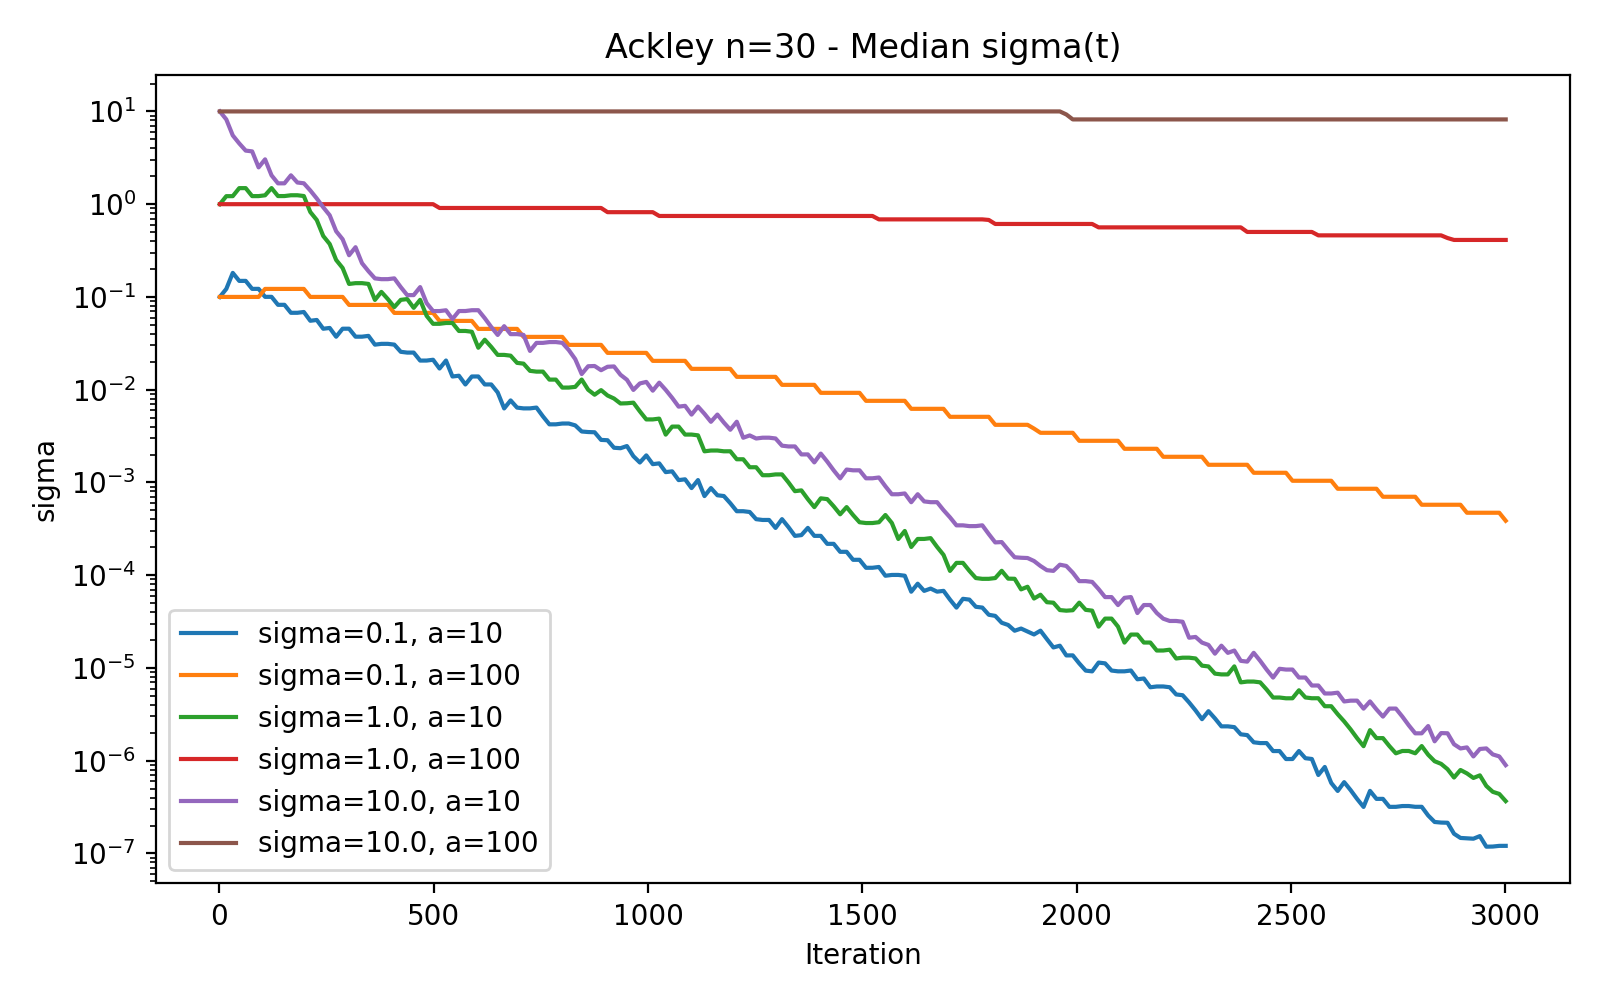
\includegraphics[width=\textwidth]{charts/Ackley_n30_all_sigmas.png}\\
        \small Mediany $\sigma(t)$
    \end{minipage}
    \caption{Mediany $f(t)$ oraz $\sigma(t)$ dla funkcji Ackleya ($n=30$) dla różnych $\sigma$ i $a$.}
\end{figure}

\newpage
\section{Podsumowanie}
Przeprowadzone eksperymenty pozwalają na analizę wpływu parametrów $\sigma$ i $a$ na efektywność optymalizacji. Wartości median $f(t)$ oraz $\sigma(t)$ umożliwiają porównanie stabilności i szybkości zbieżności algorytmu dla różnych ustawień. Szczegółowe wnioski można wyciągnąć na podstawie kształtu i przebiegu wykresów.

\subsection*{Wnioski szczegółowe}
\textbf{Funkcja kwadratowa:} \\
Najlepszy wynik dla funkcji kwadratowej otrzymaliśmy dla $\sigma=0.1$ i $a=10$ (zarówno dla $n=10$, jak i $n=30$). Wartość funkcji celu była bardzo zbliżona do minimum globalnego.

\textbf{Funkcja Ackleya:} \\
Najlepszy wynik dla funkcji Ackleya otrzymaliśmy dla $\sigma=1$ i $a=100$ dla $n=10$ (wartość funkcji celu ok. 3{,}8) oraz dla $\sigma=10$ i $a=10$ dla $n=30$ (wartość funkcji celu ok. 5{,}5). Poszukiwania minimów globalnych często utknęły w minimach lokalnych, jednak w pojedynczych testach udało się osiągnąć minimum globalne dla $n=10$. Dla wyższych wartości $a$ funkcja Ackleya jest bardziej skłonna znajdować minima globalne z uwagi na rzadszą korektę wartości $\sigma$, co skutkuje większymi skokami wartości funkcji celu.

\textbf{Funkcja Rosenbrocka:} \\
Najlepszy wynik funkcji celu uzyskano dla $\sigma=0.1$ i $a=10$. Dla $n=10$ wartość funkcji celu wynosiła ok. 10, a dla $n=30$ ok. 12. Poszukiwania minimów globalnych również utknęły w minimach lokalnych.

\newpage
\section{Zależność przebiegu $\sigma(t)$ od funkcji i parametrów}
Parametr $\sigma$ w algorytmie steruje rozrzutem mutacji, a więc decyduje o intensywności eksploracji przestrzeni rozwiązań. Jego przebieg w czasie zależy zarówno od charakteru funkcji celu, jak i od ustawień parametrów $a$ (częstotliwość korekty) oraz wartości początkowej $\sigma$.

\textbf{Funkcja kwadratowa:} \\
Dla funkcji kwadratowej $\sigma(t)$ zwykle szybko stabilizuje się na pewnym poziomie, a wahania są niewielkie. Wynika to z prostoty krajobrazu funkcji i łatwości poprawy rozwiązania.

\textbf{Funkcja Rosenbrocka:} \\
Dla funkcji Rosenbrocka $\sigma$ często systematycznie maleje, ponieważ poprawa rozwiązania jest trudniejsza, a algorytm rzadziej odnosi sukcesy. Przebieg $\sigma(t)$ jest bardziej wrażliwy na parametry $a$ i wartość początkową $\sigma$.

\textbf{Funkcja Ackleya:} \\
Dla funkcji Ackleya $\sigma(t)$ może długo oscylować, szczególnie przy dużych wartościach $a$. Często obserwuje się zarówno okresy wzrostu, jak i spadku $\sigma$, co jest efektem utkwienia w minimach lokalnych i prób ich opuszczenia. Przy dużych $a$ korekty są rzadsze, co skutkuje większymi skokami wartości $\sigma$.

\textbf{Wpływ parametrów:}
\begin{itemize}
    \item Małe $a$ (np. 10): częstsza korekta $\sigma$, mniejsze skoki, większa stabilność przebiegu.
    \item Duże $a$ (np. 100): rzadsza korekta, większe skoki, większa szansa na ucieczkę z minimum lokalnego, ale też większa niestabilność.
    \item Mała wartość początkowa $\sigma$: eksploracja lokalna, szybka stabilizacja.
    \item Duża wartość początkowa $\sigma$: większa eksploracja, ale ryzyko przeskakiwania minimum.
\end{itemize}

Podsumowując, optymalny przebieg $\sigma(t)$ zależy od charakteru funkcji celu oraz dobranych parametrów. Dla funkcji o prostym krajobrazie (kwadratowa) preferowane są mniejsze i stabilne wartości $\sigma$, natomiast dla funkcji z wieloma minimami lokalnymi (Ackley, Rosenbrock) korzystne mogą być większe i bardziej dynamiczne zmiany $\sigma$.

\end{document}
